\documentclass[12pt,a4paper]{report}
\usepackage[utf8]{inputenc}
\usepackage[T1]{fontenc}
\usepackage{amsmath,amssymb}
\usepackage{booktabs,longtable,array,multirow}
\usepackage{graphicx,float,caption,subcaption}
\usepackage{geometry,setspace,parskip,enumitem,xcolor}
\usepackage{hyperref,cleveref,fancyhdr,titlesec,tocloft}
\usepackage{pgfplots,tikz}
\pgfplotsset{compat=1.18}
\usetikzlibrary{shapes.geometric,arrows.meta,positioning,calc,patterns,fit,backgrounds}
\usepackage{listings}

\definecolor{codeblue}{rgb}{0.13,0.29,0.53}
\definecolor{codegreen}{rgb}{0.0,0.45,0.0}
\definecolor{backcolour}{rgb}{0.97,0.97,0.97}
\definecolor{hitblue}{RGB}{0,51,102}
\definecolor{accentblue}{RGB}{41,128,185}
\definecolor{lightgray}{RGB}{236,240,241}
\definecolor{darkgray}{RGB}{44,62,80}
\definecolor{lavender}{RGB}{200,200,240}

\lstdefinestyle{pythonstyle}{
  language=Python, backgroundcolor=\color{backcolour},
  commentstyle=\color{codegreen}, keywordstyle=\color{codeblue}\bfseries,
  basicstyle=\ttfamily\footnotesize, breaklines=true,
  numbers=left, numbersep=5pt, frame=single, showstringspaces=false,
}

\geometry{left=1.5in,right=1in,top=1in,bottom=1in}
\onehalfspacing

\pagestyle{fancy}\fancyhf{}
\fancyhead[R]{\thepage}
\fancyhead[L]{\nouppercase{\leftmark}}
\renewcommand{\headrulewidth}{0.4pt}

\titleformat{\chapter}[display]
  {\normalfont\huge\bfseries}
  {\chaptertitlename\ \thechapter}
  {20pt}
  {\Huge\bfseries}

\titleformat{\section}{\normalfont\Large\bfseries}{\thesection}{1em}{}
\titleformat{\subsection}{\normalfont\large\bfseries}{\thesubsection}{1em}{}
\titleformat{\subsubsection}{\normalfont\normalsize\bfseries}{\thesubsubsection}{1em}{}

\hypersetup{colorlinks=true,linkcolor=blue,urlcolor=cyan,citecolor=blue,
  pdftitle={Pension Fund Efficiency Toolkit: Prototype Documentation},
  pdfauthor={Lorraine Mujuru}}

\begin{document}

%% ── COVER PAGE ───────────────────────────────────────────────
\thispagestyle{empty}
\begin{center}

\includegraphics[width=0.8\textwidth]{../../../document/hit_logo.png}\\[0.3cm]
{\normalsize\bfseries SCHOOL OF BUSINESS AND MANAGEMENT SCIENCES}\\[0.2cm]
{\normalsize\bfseries DEPARTMENT OF FINANCIAL ENGINEERING}\\[1.5cm]
{\normalsize\bfseries PENSION FUND EFFICIENCY TOOLKIT: A PROTOTYPE SYSTEM FOR
FRONTIER-BASED OPTIMIZATION ANALYSIS OF SELF-ADMINISTERED PENSION FUNDS IN ZIMBABWE}\\[1.5cm]
{\normalsize BY}\\[0.5cm]
{\large\bfseries LORRAINE MUJURU}\\[0.2cm]
{\large\bfseries H220021Y}\\[1cm]
{\normalsize\bfseries SUPERVISOR: MR SHUMBASHAVA}\\[1cm]
{\small THIS PROTOTYPE DOCUMENTATION IS SUBMITTED TO THE DEPARTMENT OF FINANCIAL
ENGINEERING, SCHOOL OF BUSINESS AND MANAGEMENT SCIENCES, IN PARTIAL FULFILMENT
OF THE BACHELOR OF TECHNOLOGY HONOURS DEGREE IN FINANCIAL ENGINEERING}\\[1cm]
{\large\bfseries 2026}
\end{center}
\newpage

%% ── FRONT MATTER (roman numerals) ────────────────────────────
\pagenumbering{roman}

%% TITLE PAGE
\chapter*{Title Page}
\addcontentsline{toc}{chapter}{Title Page}

\begin{tabbing}
\hspace{4.5cm}\=\kill
\textbf{Title of project:}   \> PENSION FUND EFFICIENCY TOOLKIT \\[1em]
\textbf{Author:}             \> LORRAINE MUJURU \\[1em]
\textbf{University Name:}    \> HARARE INSTITUTE OF TECHNOLOGY \\[1em]
\textbf{School Name:}        \> BUSINESS AND MANAGEMENT SCIENCES \\[1em]
\textbf{Department Name:}    \> DEPARTMENT OF FINANCIAL ENGINEERING \\[1em]
\textbf{Year:}               \> 2026 \\
\end{tabbing}
\newpage

%% DECLARATION
\chapter*{Declaration}
\addcontentsline{toc}{chapter}{Declaration}

I the author, LORRAINE MUJURU H220021Y do hereby declare that this work has not
previously been accepted in substance for any degree and is not being concurrently
submitted in candidature for any degree.

\vspace{3cm}
Student Signature\dotfill Date\dotfill

\vspace{2.5cm}
Supervisor's Signature\dotfill Date\dotfill
\newpage

%% COPYRIGHT
\chapter*{Copyright}
\addcontentsline{toc}{chapter}{Copyright}

All rights reserved. No part of this research may be reproduced, stored in any
retrieval system, or transmitted in any form or by any means, electronic, mechanical,
photocopying, recording or otherwise from scholarly purpose without the prior written
permission of the author and Harare Institute of Technology on behalf of the author.
\newpage

%% DEDICATION
\chapter*{Dedication}
\addcontentsline{toc}{chapter}{Dedication}

This prototype is dedicated to my family, whose unwavering support throughout my
studies at HIT made this work possible. The sacrifices they made and the encouragement
they offered during difficult periods are what carried me to the finish line. I hope this
achievement brings them the pride they deserve.
\newpage

%% ACKNOWLEDGEMENTS
\chapter*{Acknowledgements}
\addcontentsline{toc}{chapter}{Acknowledgements}

I would like to extend sincere gratitude to my supervisor for the guidance and mentorship
provided throughout the development of this prototype. The constructive feedback at each
stage of the project meaningfully shaped both the quality and direction of the final system.

My appreciation also goes to the Department of Financial Engineering and the research
coordinators whose continued support during the final year kept the project on track. Their
direction was particularly valuable during the more demanding phases of implementation.

Lastly, I thank my fellow students and friends at HIT. Four years of shared experiences,
late-night study sessions, and diverse perspectives have had a genuine impact on who I am
as both a student and a person.
\newpage

%% TABLE OF CONTENTS
\tableofcontents
\newpage

%% LIST OF FIGURES
\listoffigures
\newpage

%% LIST OF TABLES
\listoftables
\newpage

%% ABSTRACT
\chapter*{Abstract}
\addcontentsline{toc}{chapter}{Abstract}

The Pension Fund Efficiency Toolkit is a software prototype that operationalises the
analytical framework from the accompanying research study on frontier-based efficiency
measurement of Zimbabwean self-administered pension funds. The system translates a
multi-stage pipeline --- covering data ingestion, efficiency scoring, peer benchmarking,
and contextual factor analysis --- into an interactive web-based dashboard designed for
pension fund managers. Built in Python~3.11 using Streamlit and a set of specialised
open-source libraries, the prototype enables users to upload fund data, execute the full
analysis pipeline without any programming knowledge, and generate professional PDF reports
suitable for board presentations and regulatory submissions. The system demonstrates that
rigorous financial modelling can be made accessible to non-technical practitioners through
careful interface design without sacrificing analytical integrity.
\newpage

%% ABBREVIATIONS
\chapter*{Abbreviation}
\addcontentsline{toc}{chapter}{Abbreviation}

\begin{table}[H]
\centering
\begin{tabular}{|l|l|}
\hline
\textbf{Abbreviation} & \textbf{Full Form} \\
\hline
DEA   & Data Envelopment Analysis \\
\hline
CCR   & Charnes, Cooper and Rhodes Model \\
\hline
BCC   & Banker, Charnes and Cooper Model \\
\hline
CRS   & Constant Returns to Scale \\
\hline
VRS   & Variable Returns to Scale \\
\hline
IRS   & Increasing Returns to Scale \\
\hline
DRS   & Decreasing Returns to Scale \\
\hline
RF    & Random Forest \\
\hline
PDF   & Portable Document Format \\
\hline
UI    & User Interface \\
\hline
IPEC  & Insurance and Pensions Commission \\
\hline
HIT   & Harare Institute of Technology \\
\hline
SQLite & Self-Contained Relational Database Engine \\
\hline
CSV   & Comma-Separated Values \\
\hline
\end{tabular}
\caption{Glossary of Abbreviations}
\label{tab:abbrev}
\end{table}
\newpage

%% ── MAIN MATTER (arabic numerals) ────────────────────────────
\pagenumbering{arabic}

%%=============================================================
%% CHAPTER 1: INTRODUCTION
%%=============================================================
\chapter{INTRODUCTION}

Zimbabwe's pension sector has faced considerable turbulence over the past decade.
Hyperinflation eroded fund values substantially, exchange rate instability disrupted
investment portfolios, and regulatory scrutiny intensified following several high-profile
fund failures. Against this backdrop pension fund managers need practical tools --- not
just academic models --- to understand how efficiently their funds are operating and where
improvements are realistically achievable.

The Pension Fund Efficiency Toolkit is the software implementation of a research study on
efficiency measurement in Zimbabwe's self-administered standalone pension funds. The study
applied Data Envelopment Analysis (DEA) to benchmark funds against each other and then
used a Random Forest regression model to identify which structural and environmental factors
drive the observed efficiency differences. This prototype takes that analytical pipeline from
a research setting into practice, packaging it into an interactive dashboard that a fund
manager can actually sit down and use. No programming is required.

The system processes panel data from up to twenty registered Zimbabwean pension funds.
It produces efficiency scores, identifies top-performing peer funds, generates specific
cost-reduction recommendations, and exports formatted PDF reports. All of this happens
through a web interface accessible from a standard browser.

\section{Problem Statement}

Pension fund managers in Zimbabwe currently lack accessible tools to systematically
evaluate operational efficiency. Regulators like the Insurance and Pensions Commission
(IPEC) collect annual financial disclosures, but there is no standardised mechanism for
funds to benchmark themselves against peers or receive specific, data-driven guidance on
improving performance. Those who want to understand their fund's relative position typically
rely on manual spreadsheet comparisons --- time-consuming work that is prone to error and
fails to capture the multi-dimensional nature of fund performance.

The analytical framework that addresses these limitations --- Data Envelopment Analysis ---
computes a frontier of best-practice performance across the peer group and measures each
fund's distance from that frontier. DEA and its extensions have historically been the domain
of researchers. The gap between what the literature makes available and what fund managers
can practically access is exactly what motivated the development of this system.

\section{System Objectives}

The Pension Fund Efficiency Toolkit was designed to achieve the following objectives:

\begin{itemize}
  \item To implement a fund efficiency scoring pipeline that evaluates both overall and
        internal operational efficiency for up to twenty Zimbabwean pension funds

  \item To automatically identify best-practice benchmark funds and calculate specific,
        actionable input-reduction targets for underperforming funds in dollar terms

  \item To determine which structural and environmental factors most strongly influence
        fund efficiency across the sector as a whole

  \item To deliver an interactive browser-based dashboard requiring no technical expertise
        to operate, so that fund managers can run the full analysis independently

  \item To persist uploaded fund data in a local database so that managers do not need to
        re-upload files on subsequent visits

  \item To generate downloadable PDF reports summarising findings for stakeholders and
        regulatory purposes
\end{itemize}

\subsection*{Conclusion}

This chapter established the sector context and motivation behind the prototype.
Zimbabwe's pension funds operate in a difficult environment and evidence-based efficiency
measurement can help managers make better decisions with the resources they have. The
objectives show that the system aims to bridge the gap between research-grade analytical
methods and practical day-to-day fund management. The chapters that follow document the
development process, feasibility considerations, and the full system implementation.

%%=============================================================
%% CHAPTER 2: PROCESS MODELLING
%%=============================================================
\chapter{PROCESS MODELLING}

\section{Introduction}

Building this prototype meant choosing a development approach that could accommodate both
the technical complexity of the underlying analytical models and the requirement that the
resulting interface be simple for non-technical users to operate. This chapter covers the
process model chosen, a feasibility analysis across four dimensions, and the security
architecture that governs system access.

\section{Process Model (Iterative)}

\begin{figure}[H]
\centering
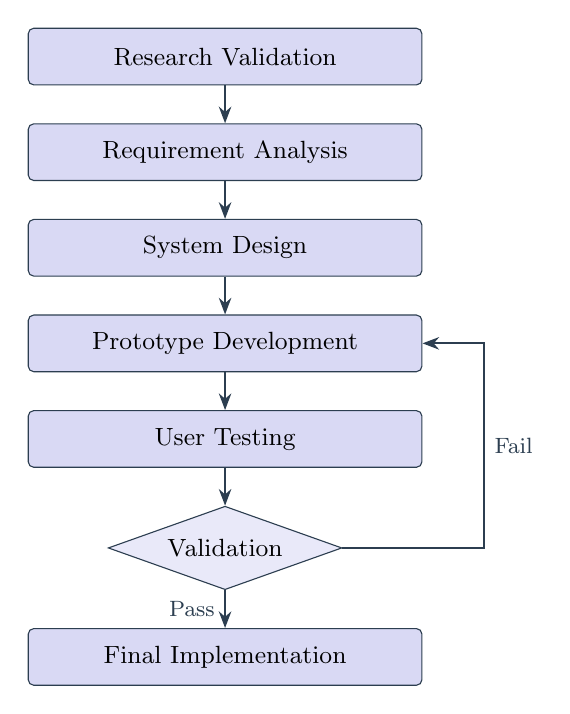
\begin{tikzpicture}[
  proc/.style={rectangle, draw=darkgray, fill=lavender!70, text centered,
               minimum width=5cm, minimum height=0.72cm, font=\small, rounded corners=2pt},
  dec/.style={diamond, draw=darkgray, fill=lavender!40, aspect=2.8,
              text centered, font=\small},
  arr/.style={-{Stealth[length=6pt]}, thick, darkgray},
  node distance=0.48cm, every node/.style={align=center}
]
\node[proc](rv){Research Validation};
\node[proc,below=of rv](ra){Requirement Analysis};
\node[proc,below=of ra](sd){System Design};
\node[proc,below=of sd](pd){Prototype Development};
\node[proc,below=of pd](ut){User Testing};
\node[dec,below=of ut](vl){Validation};
\node[proc,below=of vl](fi){Final Implementation};

\draw[arr](rv)--(ra);
\draw[arr](ra)--(sd);
\draw[arr](sd)--(pd);
\draw[arr](pd)--(ut);
\draw[arr](ut)--(vl);
\draw[arr](vl)--node[left,font=\footnotesize]{Pass}(fi);
\draw[arr](vl.east)--++(1.8,0)|-node[right,font=\footnotesize,pos=0.25]{Fail}(pd.east);
\end{tikzpicture}
\caption{Process Model (Iterative)}
\label{fig:process_model}
\end{figure}

The iterative prototyping model was selected for this project for several reasons.
Financial analysis software of this kind depends on tight feedback loops between the
analytical engine and the interface. Getting the DEA pipeline to produce correct results is
one thing; surfacing those results in a way that a fund manager actually finds interpretable
is quite another. Iterative development allowed both concerns to be addressed in cycles
rather than requiring a complete design commitment upfront.

The approach also suited the nature of the underlying algorithms. The bootstrap
bias-correction module and the Random Forest second-stage analysis each required
calibration iterations. Being able to revisit the design of these components after
observing their outputs in the dashboard context --- rather than validating them in
isolation --- produced a more coherent final product. Each cycle of the model above maps
roughly to one development sprint, with the validation step corresponding to functional
testing of the dashboard against expected analytical outputs.

\section{Feasibility Analysis}

\begin{itemize}
  \item \textbf{Economic Feasibility}: The entire system is built on open-source
  technologies. Python, Streamlit, PuLP, scikit-learn, and SQLite carry no licensing
  costs. Compared to commercial financial analytics platforms that charge per-seat fees
  running into thousands of dollars annually, this prototype achieves equivalent
  functionality at essentially zero cost while being tailored specifically to the
  Zimbabwean pension context.

  \item \textbf{Technical Feasibility}: The DEA linear programmes solve in milliseconds
  per fund using the PuLP/CBC solver on standard hardware. The bootstrap procedure ---
  which runs two hundred or more resampling iterations to produce statistically valid
  efficiency estimates --- completes in under a minute for nineteen funds on a modern
  laptop. Streamlit handles the web interface without requiring a dedicated server; a
  single command launches the application locally, making deployment straightforward even
  where IT infrastructure is limited.

  \item \textbf{Social Feasibility}: Pension fund managers are not, in general,
  quantitative analysts. The dashboard design reflects this reality. Efficiency scores are
  expressed as percentages with plain-English status labels (Excellent, Good, Fair, Needs
  Attention), recommendations are stated as specific dollar amounts rather than technical
  slack values, and academic terminology is kept away from the interface entirely. The
  system was refined iteratively to ensure that outputs are interpretable without any
  background in DEA or statistics.

  \item \textbf{Operational Feasibility}: The system accepts CSV files in a format
  consistent with data that fund managers already compile for IPEC submissions. No
  infrastructure changes are required on the user's side. The built-in SQLite database
  means that uploaded data persists between sessions, so a manager does not need to
  re-upload the same dataset each time they log in. The application runs locally on a
  Windows or Linux machine with Python installed.
\end{itemize}

\section{System Security}

Access to the system is controlled by credential-based login. The administrator account
representing the fund manager is configured through environment variables rather than
being stored in the database, which means the primary credentials are never written to disk
in plain text form. The password is managed solely by the system developer and the
designated user.

The application does not expose any network endpoints beyond the local machine by default.
All fund data is stored in a local SQLite file rather than on a remote server, reducing
the attack surface considerably. The security model is intentionally simple and
proportionate to the single-user deployment context: there is one authenticated user, and
unauthenticated sessions are immediately redirected to the login page.

\subsection*{Conclusion}

Through iterative development the prototype successfully addressed the gap between
research-grade analysis and practical day-to-day use. The feasibility study confirms that
the system is economically viable, technically sound, socially appropriate for its intended
users, and operationally compatible with existing workflows in Zimbabwean pension fund
management. The security architecture is straightforward and appropriate for the deployment
context.

%%=============================================================
%% CHAPTER 3: SOFTWARE METHODOLOGY
%%=============================================================
\chapter{SOFTWARE METHODOLOGY}

\section{Introduction}

This chapter describes the implementation of the Pension Fund Efficiency Toolkit at the
system level. It covers the overall flow of the application from the user's perspective,
describes each screen and its purpose, and provides representative code extracts from the
core modules. The aim is to give a clear picture of how the system works from the front
end all the way through to the data layer.

\section{System Flowchart}

\begin{figure}[H]
\centering
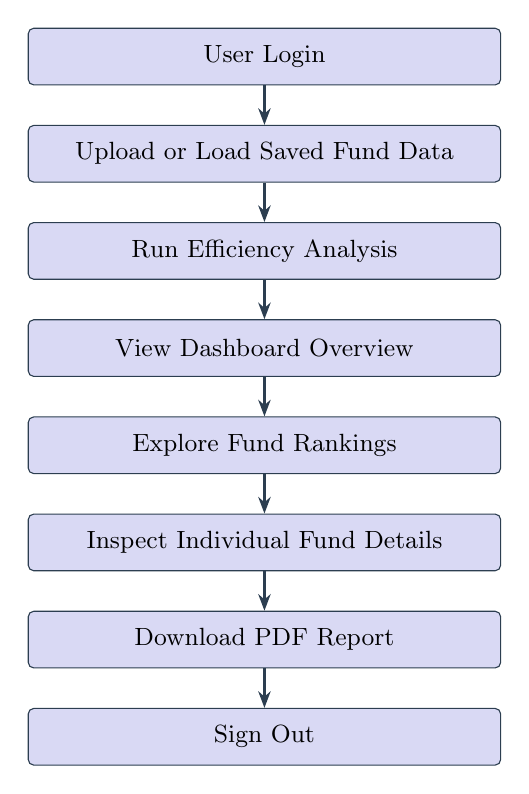
\begin{tikzpicture}[
  proc/.style={rectangle, draw=darkgray, fill=lavender!70, text centered,
               minimum width=6cm, minimum height=0.72cm, font=\small, rounded corners=2pt},
  arr/.style={-{Stealth[length=6pt]}, thick, darkgray},
  node distance=0.5cm, every node/.style={align=center}
]
\node[proc](login){User Login};
\node[proc,below=of login](load){Upload or Load Saved Fund Data};
\node[proc,below=of load](run){Run Efficiency Analysis};
\node[proc,below=of run](dash){View Dashboard Overview};
\node[proc,below=of dash](rank){Explore Fund Rankings};
\node[proc,below=of rank](detail){Inspect Individual Fund Details};
\node[proc,below=of detail](report){Download PDF Report};
\node[proc,below=of report](logout){Sign Out};

\draw[arr](login)--(load);
\draw[arr](load)--(run);
\draw[arr](run)--(dash);
\draw[arr](dash)--(rank);
\draw[arr](rank)--(detail);
\draw[arr](detail)--(report);
\draw[arr](report)--(logout);
\end{tikzpicture}
\caption{System Flowchart}
\label{fig:sys_flowchart}
\end{figure}

The flowchart maps the primary use path through the application. When a user authenticates,
the system checks whether they have any previously uploaded datasets saved in the local
database and loads the most recent one automatically --- so returning users land directly
on the dashboard without needing to re-upload anything. If no saved data exists, the CSV
upload widget in the sidebar is used. Clicking Run Analysis triggers the full pipeline:
CCR efficiency scoring, BCC efficiency scoring, scale efficiency classification, bootstrap
bias correction, and the Random Forest second-stage determinant analysis. Results are
stored in the session and the tabbed dashboard allows exploration at whatever level of
detail the manager needs.

\section{System Description}

\subsection{Step 1: Login}

\begin{figure}[H]
\centering
\fbox{%
\parbox{0.68\textwidth}{%
\vspace{0.5cm}
\centering
{\large\bfseries\textcolor{hitblue}{Pension Efficiency Toolkit}}\\[0.1cm]
{\small Zimbabwe Pension Fund Analysis System}\\[0.6cm]
\begin{tabular}{p{0.58\textwidth}}
\textbf{Email Address}\\[0.15cm]
\framebox[0.56\textwidth]{\phantom{your.email@example.com}}\\[0.4cm]
\textbf{Password}\\[0.15cm]
\framebox[0.56\textwidth]{\phantom{\ \ \ \ \ \ \ \ \ \ \ \ \ \ }}\\[0.5cm]
\framebox[0.56\textwidth]{\centering\textbf{Sign In}}\\[0.3cm]
\end{tabular}
\vspace{0.3cm}%
}}
\caption{Login Screen}
\label{fig:login}
\end{figure}

The login screen is the system's entry point. The user enters their email address and
password. Authentication is handled against credentials stored in environment variables on
the server side --- the fund manager's email and password are set at deployment time and are
never held in the database. Failed attempts return a clear error message; successful login
redirects to the main dashboard immediately.

\subsection{Launch Page --- Dashboard Overview}

\begin{figure}[H]
\centering
\fbox{%
\parbox{0.82\textwidth}{%
\vspace{0.3cm}
\small
\textbf{\textcolor{hitblue}{Pension Fund Efficiency Dashboard}}\\
{\footnotesize Helping Zimbabwe's pension funds operate at their best}\\[0.3cm]
\begin{tabular}{|p{2.1cm}|p{2.1cm}|p{2.1cm}|p{2.1cm}|}
\hline
\small\textbf{Funds Analysed} & \small\textbf{Sector Average} &
\small\textbf{Top Performer}  & \small\textbf{Need Attention}  \\
\hline
\centering\small 19 & \centering\small 78\% & \centering\small POSB Staff Pension & \centering\small 5\tabularnewline
\hline
\end{tabular}\\[0.4cm]
\textit{[Ranked horizontal bar chart --- Fund Efficiency Rankings]}\\[0.25cm]
\textit{[Sector Insight summary box with estimated sector savings]}\\
\vspace{0.3cm}%
}}
\caption{Dashboard Overview}
\label{fig:dashboard}
\end{figure}

After login the user arrives at the main dashboard. The sidebar shows any previously saved
datasets and allows a new CSV upload. Once data is loaded and Run Analysis is clicked, the
overview tab displays four headline metrics: number of funds analysed, sector average
efficiency, the top-performing fund, and how many funds fall below the 75\,\% threshold.
A ranked horizontal bar chart shows all funds by efficiency score, colour-coded from red
through orange to green. At the bottom a plain-language insight box summarises the sector
picture and estimates total annual savings available if underperforming funds reached
the efficiency frontier.

\subsection{Fund Rankings}

\begin{figure}[H]
\centering
\fbox{%
\parbox{0.82\textwidth}{%
\vspace{0.3cm}
\small
\textbf{Fund Performance Rankings}\\[0.15cm]
{\footnotesize Every fund is scored on how efficiently it converts resources into returns
for members. A score of 100\% means the fund is on the frontier.}\\[0.3cm]
{\footnotesize
\begin{tabular}{|p{0.6cm}|p{3.5cm}|p{1.2cm}|p{1.5cm}|p{1.5cm}|}
\hline
\textbf{\#} & \textbf{Fund Name} & \textbf{Score} & \textbf{Status} &
\textbf{Savings}\\
\hline
1  & POSB Staff Pension Fund           & 100.0\% & Excellent &  ---   \\
2  & Zimplats Mineworkers Pension      &  98.3\% & Excellent &  ---   \\
3  & Delta Corporation Pension         &  91.5\% & Excellent & \$1.2M \\
\ldots & \ldots & \ldots & \ldots & \ldots \\
\hline
\end{tabular}
}\\[0.35cm]
\textit{[Scatter plot: Overall Efficiency vs.\ Internal Efficiency]}\\
\vspace{0.3cm}%
}}
\caption{Fund Rankings Tab}
\label{fig:rankings}
\end{figure}

The rankings tab presents a full table of all funds ordered by efficiency score. Each row
shows rank, fund name, score, status label, and estimated annual savings potential. Below
the table a scatter plot compares overall efficiency against internal operational
efficiency. This helps distinguish funds that are simply operating at the wrong scale from
those with genuine operational inefficiencies. Funds sitting on the diagonal line have
matching scores across both measures.

\subsection{Fund Details}

\begin{figure}[H]
\centering
\fbox{%
\parbox{0.82\textwidth}{%
\vspace{0.3cm}
\small
\textbf{Select a Fund to View:}\ \
\framebox[5cm]{CBZ Bank Staff Pension Fund \quad$\vee$}\\[0.4cm]
\begin{tabular}{p{3.6cm}p{7.5cm}}
\textit{[Gauge: 68\%]} &
\textbf{CBZ Bank Staff Pension Fund}\\[0.15cm]
& Ranked 12 of 19 funds\\[0.25cm]
& Efficiency Score: 68.0\% \quad|\quad Sector Average: 78\%\\
& Gap to Average: $-$10.0\%\\[0.3cm]
& \textcolor{orange}{\small\textit{This fund is underperforming relative to
its peers.}}\\
\end{tabular}\\[0.35cm]
\textbf{Recommended Actions:}\\[0.1cm]
{\small Reduce Operating Expenses: \$3.4M $\to$ \$2.1M \quad(saves \$1.3M/year)}\\[0.1cm]
\textbf{Learn From:} POSB Staff Pension Fund \quad|\quad Zimplats Mineworkers Pension Fund\\
\vspace{0.25cm}%
}}
\caption{Fund Details Tab}
\label{fig:fund_details}
\end{figure}

This tab lets the manager select any individual fund and drill into its performance. A
gauge chart shows the efficiency score visually, with colour zones running from red at the
bottom to green at the top. To the right the fund's rank, score relative to the sector
average, and a plain-language interpretation are displayed. Below the gauge, specific
recommendations list each input where a reduction is achievable, showing the current
amount, the recommended target, and the estimated annual saving. A peer benchmarking
section at the bottom identifies the most similar high-performing funds so the manager can
investigate what those funds do differently in practice.

\subsection{Download Report}

\begin{figure}[H]
\centering
\fbox{%
\parbox{0.72\textwidth}{%
\vspace{0.4cm}
\small
\textbf{Download Full Analysis Report}\\[0.25cm]
{\footnotesize The PDF report includes efficiency scores for all funds, input reduction
targets, the rankings table, and key findings. Suitable for stakeholder presentations and
regulatory submissions.}\\[0.5cm]
\hspace{1cm}\framebox[5.5cm]{\centering\textbf{Generate PDF Report}}\\[0.4cm]
\hspace{1cm}\framebox[5.5cm]{\centering\textbf{Download Report (PDF)}}\\
\vspace{0.4cm}%
}}
\caption{Download Report Tab}
\label{fig:report_tab}
\end{figure}

The reports tab provides a single button that generates a formatted PDF report using
ReportLab. The document includes an executive summary, the complete efficiency rankings
table, scale efficiency classifications, input reduction targets for each fund, and a
feature importance chart showing which factors most influence fund efficiency across the
sector. Once generated, a download button appears so the file can be saved locally.

\newpage
\noindent\textbf{\large APPENDIX}
\vspace{0.5cm}

\subsection{System Code}

The authentication module verifies the fund manager's credentials against environment
variables. Because credentials are never stored in the database, there is no risk of
plaintext password exposure in the SQLite file.

\begin{lstlisting}[style=pythonstyle, caption={Login credential verification --- auth.py}]
def login(email: str, password: str) -> tuple[bool, str, bool, int]:
    """Attempt login. Returns (success, display_name, is_admin, user_id)."""
    from pension_toolkit.db import ADMIN_USER_ID, get_user_by_email

    email = email.strip()

    # Admin credentials come from environment variables, never the database
    if is_admin_email(email):
        if password == _admin_password():
            return True, _admin_name(), True, ADMIN_USER_ID
        return False, "", False, -1

    user = get_user_by_email(email)
    if user and user["password"] == password:
        return True, user["full_name"], False, user["id"]
    return False, "", False, -1
\end{lstlisting}

The pipeline function aggregates multi-year panel data to a cross-sectional representation
and then orchestrates the DEA solver, scale analysis, bootstrap procedure, and Random
Forest second stage in sequence.

\begin{lstlisting}[style=pythonstyle, caption={Analysis pipeline --- ui\_streamlit.py}]
def run_pipeline(df: pd.DataFrame, B: int, seed: int) -> dict:
    numeric_cols = df.select_dtypes(include="number").columns.tolist()
    df_agg = df.groupby("fund_id")[numeric_cols].mean().reset_index()
    fund_name_map = df.groupby("fund_id")["fund_name"].agg(
        lambda x: x.mode()[0])
    df_agg = df_agg.merge(fund_name_map, on="fund_id")

    X_in, Y_out, fund_ids = get_dea_matrices(df_agg, INPUT_COLS, OUTPUT_COLS)
    ccr   = dea_ccr_input_oriented(X_in, Y_out, fund_ids)
    bcc   = dea_bcc_input_oriented(X_in, Y_out, fund_ids)
    scale = compute_scale_efficiency(ccr, bcc)

    def _ccr_func(X, Y):
        return dea_ccr_input_oriented(X, Y, fund_ids)

    boot = simar_wilson(_ccr_func, X_in, Y_out,
                        fund_ids=fund_ids, B=B, seed=seed)

    ...
    return dict(ccr=ccr, bcc=bcc, scale_df=scale_df,
                boot_df=boot_df, rf_result=rf_result, ...)
\end{lstlisting}

The data persistence layer stores every CSV upload with its fund data rows so that results
survive browser restarts. The upload history table allows the manager to switch between
multiple datasets without re-uploading.

\begin{lstlisting}[style=pythonstyle, caption={Fund data persistence --- db.py}]
def save_fund_data(df: pd.DataFrame, filename: str, user_id: int) -> int:
    """Persist a new upload for the given user. Returns the new upload_id."""
    with _connect() as conn:
        _init_tables(conn)
        n_rows  = len(df)
        n_funds = int(df["fund_id"].nunique())
        uploaded_at = datetime.now().isoformat(timespec="seconds")

        cur = conn.execute(
            "INSERT INTO upload_history "
            "(user_id, filename, uploaded_at, n_rows, n_funds) "
            "VALUES (?, ?, ?, ?, ?)",
            (user_id, filename, uploaded_at, n_rows, n_funds),
        )
        upload_id = cur.lastrowid
        df_to_save = df.copy()
        df_to_save["upload_id"] = upload_id
        df_to_save.to_sql("fund_data", conn,
                          if_exists="append", index=False)
        return upload_id
\end{lstlisting}

\subsection*{Conclusion}

The implemented methodology translates the research's analytical framework into working
operational components, with each computational stage traceable to specific methods and
algorithms in the accompanying study document. The system architecture ensures all
calculations maintain analytical rigour while the user interface abstracts that complexity
into plain-language outputs that a fund manager can act on directly. The modular code
structure makes the system straightforward to maintain and extend as the dataset grows or
as future research refines the underlying methods.

\end{document}
